\subsection{Some Historical Trends}  \label{GPUArchTrends}

Figure~\ref{fig:compute-power} depicts how the aggregate compute power (GFLOPS) and the memory bandwidth (Gbps) of Nvidia GPUs has evolved from their earliest CUDA-enabled version to the current version.
Compute power has been increasing steadily at a steep slope.
Memory bandwidth has also been increasing, but not as quickly.
As a result, memory bandwidth per FLOP has been decreasing from 250 bytes/FLOP for the GTX~8800 to 41 bytes/FLOP for the GTX880.

\begin{figure}
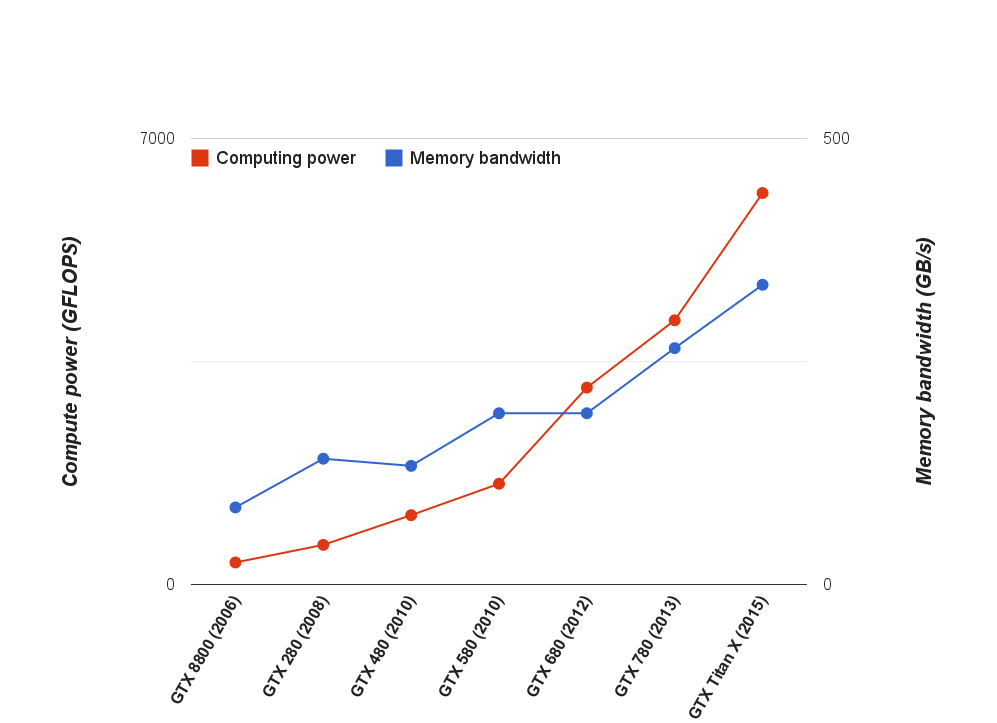
\includegraphics[width=\linewidth]{computevsmemory.png}
\caption{Compute power vs.\ memory bandwidth over time 
	\todo{add x's and years to figure}
	\todo{check if datapoints consistent with results presented in next section}
	}
\label{fig:compute-power}
\end{figure}

If this trend continues then the GPU cores will become increasingly memory starved,
considering that the number of registers are limited and the on-chip L1 cache is ineffective.
Strategies to optimize GPU applications to make more efficient use of the memory hierarchy will likely become more important going forward.

Figure~\ref{fig:memsize} depicts how the aggregate compute power and the total size of on-chip memory (L1 cache and shared memory) has evolved over time.
The total amount of on-chip memory varies over time and at one point has even decreased substantially from one generation to the next.
It has clearly not kept up with the increase in compute power. 

\begin{figure}
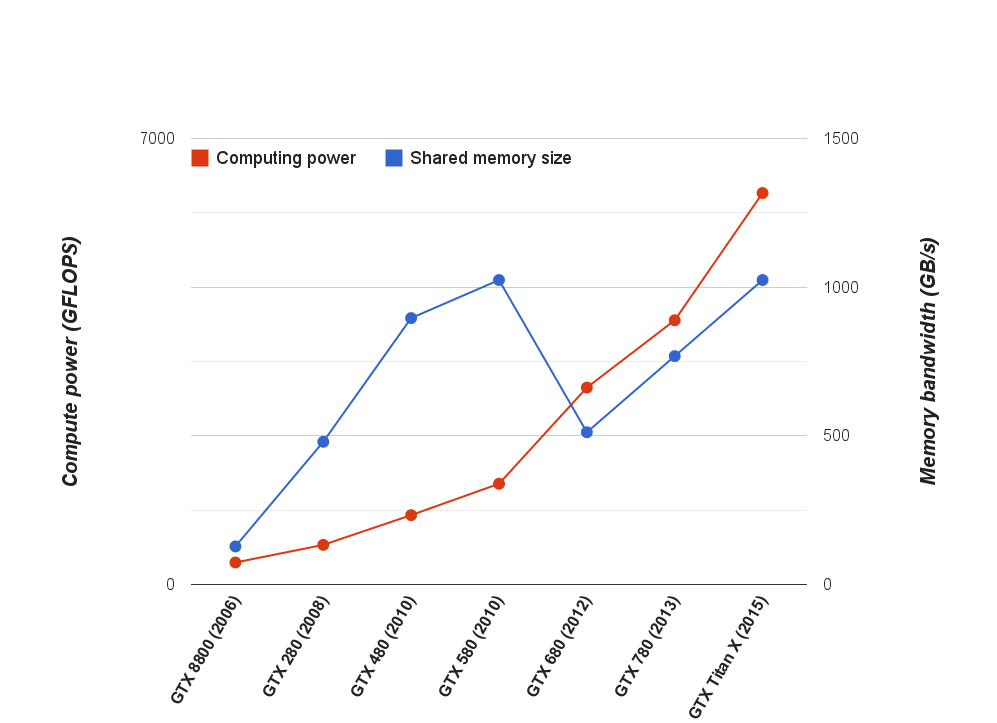
\includegraphics[width=\linewidth]{computevsshared.png}
\caption{Compute power vs.\ size of L1 and shared memory over time\todo{dito}}
\label{fig:memsize}
\end{figure}

Given the fact that future GPU generations may have smaller on-chip memory sizes, as has happened in the past, GPU programmers cannot assume the availability of a specific shared memory size.
As a result, the programmer will need to design GPU applications so that they configure the use of shared memory at run-time and possibly restrict the number of threads used by the application.
Or use run-time libraries, such as the one we are presenting in this paper, that automatically adjust program behavior to the available hardware resources.

